\documentclass{article}

\usepackage{amsmath}
\usepackage{amsfonts}
\usepackage{graphicx}
\usepackage{stmaryrd}
\usepackage{geometry}
\usepackage{float}
\usepackage{tikz}

\usetikzlibrary{shapes.geometric, arrows}
\tikzstyle{startstop} = [rectangle, rounded corners, minimum width=3cm, minimum height=1cm,text centered, draw=black, fill=gray!30]
\tikzstyle{node} = [circle, minimum width=1cm, minimum height=1cm, text centered, draw=black, fill=white]
\tikzstyle{arrow} = [thick,->,>=stealth]

\geometry{hmargin=2.5cm,vmargin=1.5cm}


\title{IEOR 240 : Homework 6}
\author{Arnaud Minondo}
\begin{document}
\maketitle
\section*{Transportation With Shortage}
Let the warehouses be respectively denoted by $W1$ and $W2$, the customers be respectively denoted by $C1$, $C2$ and $C3$.
 As there is more demand than supply I will introduce another node $S$ which will be the shortage.
 Now rename everyone following the table below : $$\begin{array}{cccccc}
    \hline
    W1 & W2 & S & C1 & C2&C3 \\\hline\hline
    1 & 2 & 3 & 4 & 5 & 6\\\hline
 \end{array}$$
Let $b = \left(\begin{array}{c}
    40\\
    30\\
    20\\
    -30\\
    -30\\
    -30\\
\end{array}\right)$, $C = \left(\begin{array}{cccccc}
    0& 0& 0 & 15& 35& 25 \\
    0& 0& 0 & 10& 50& 40 \\
    0& 0& 0 & 90& 80& 110\\
\end{array}\right)$ and $\forall i\in\{1,2,3\},j\in\{4,5,6\}, x_{ij}$ be the quantity transported from node $i$ to node $j$. With $E = \{(i,j)\in\mathbb{N}^2 \text{ s.t. } i\in\{1,2,3\},j\in\{4,5,6\}\}$ the problem can be written as :
$$\boxed{\begin{split} & \min\limits_{x_{ij}}\left(\sum\limits_{i=1}^{3}\sum\limits_{j=4}^{6}c_{ij}x_{ij}\right)\\
        &\begin{split}\text{s.t. }&\forall i\in\llbracket 1; 6\rrbracket, \sum\limits_{j|(i,j)\in E}x_{ij} - \sum\limits_{k|(k,i)\in E}x_{ki} = b_i\\
        & \forall (i,j)\in E, x_{ij}\ge 0\\
    \end{split}\\
\end{split}}$$

\section*{Shortest Path Problem}
Let nodes be $\{1,2,3,4,5,6,7,8,9,10\}$ for each possible arrival/departure day. There is always the possibility  to go from $i \in \llbracket 1;9\rrbracket $ to $j \in \llbracket i+1;10\rrbracket$ with 0 profit if you do not rent the house.
\\
Define $E = \{(i,j)\in\mathbb{N}^2\text{ s.t. } i\in\llbracket 1;9\rrbracket, j\in\llbracket i+1;10\rrbracket\}$ and $C\in\mathcal{M}_{10,10}(\mathbb{Z})$ and $b\in \mathbb{Z}^{10}$ such that : 
\\\\
$C = \left(\begin{array}{cccccccccc}
    0 & -20 & 0 & 0 & -70 & 0   &   0 & 0      & 0   & 0 \\
    0 & 0 & 0 & -20 & 0   & 0   &   0 & 0      & 0   & 0 \\
    0 & 0 & 0 & 0   & 0   & 0   & -40 & -110   & 0   & 0 \\
    0 & 0 & 0 & 0   & -10 & -60 &   0 & 0      & 0   & 0 \\
    0 & 0 & 0 & 0   &   0 & -30 &   0 & 0      & -70 & 0 \\
    0 & 0 & 0 & 0   &   0 &   0 &   0 & 0      & 0   & 0 \\
    0 & 0 & 0 & 0   &   0 &   0 &   0 & -40    & -50 & 0 \\
    0 & 0 & 0 & 0   &   0 &   0 &   0 & 0      & 0 & -30 \\
    0 & 0 & 0 & 0   &   0 &   0 &   0 & 0      & 0 &   0 \\
    0 & 0 & 0 & 0   &   0 &   0 &   0 & 0      & 0 &   0 \\
\end{array}\right)$ and $b = \left(\begin{array}{c}
    1\\
    0\\
    0\\
    0\\
    0\\
    0\\
    0\\
    0\\
    0\\
    -1\\
\end{array}\right)$
\\\\
The problem can be written as follows : $$\boxed{\begin{split}
    & \min\limits_{x_ij}\left(\sum\limits_{(i,j)\in E}c_{ij}x_{ij}\right)\\
    &\begin{split}
        \text{s.t. } & \forall i \in \llbracket 1;10\rrbracket\text{, }\sum\limits_{j|(i,j)\in E} x_{ij} - \sum\limits_{k|(k,i)\in E} x_{ki} = b_i\\
        & \forall (i,j)\in E\text{, } 0\leq x_{i,j}
    \end{split}\\
\end{split}}$$
You can refer at the graph below. For convenience I did not draw the 0 cost arrow because you can always not rent the house some days if it is more optimal. You have to consider there is always an arrow with weight 0 going from state $i$ to state $j$ for all $(i,j)\in E$
\begin{figure}[H]
    \label{label:pb4}
    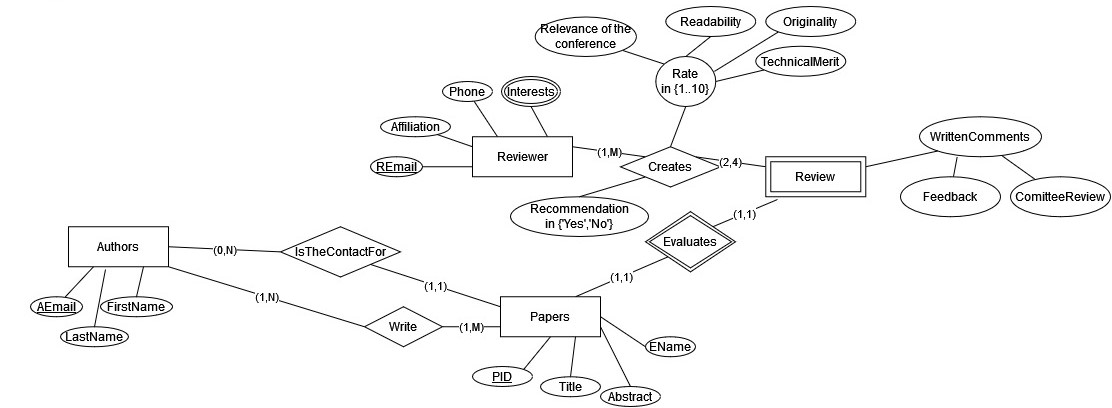
\includegraphics[height = 8cm,width = 18cm]{img/PB2.png}
    \caption{Graph of an equivalent min cost flow problem without 0 profit arrow}
\end{figure}
\section*{Set Covering Problem}
Let $x_i$ be the binary variable indicating whether siren $i$ has been installed. The ILP can be written as follows : 
$$\boxed{\begin{split}
    &\min\left(\sum_{i=1}^8x_i\right)\\
    &\begin{split}
        \text{s.t. }& x_1+x_2 = 1\\
        &x_3+x_2 \ge 1\\
        &x_4+x_5 \ge 1\\
        &x_7+x_8 \ge 1\\
        &x_7+x_6 \ge 1\\
        &x_2+x_6 \ge 1\\
        &x_1+x_6 \ge 1\\
        &x_7+x_4 \ge 1\\        
        &x_2+x_4 \ge 1\\
        &x_8+x_5 \ge 1\\
        &x_5+x_3 \ge 1\\
    \end{split}\\
\end{split}}$$
\newpage
\section*{Airplane Ticketing}
I chose to follow the hint and added for each flight 3 nodes corresponding to the three fair classes offered by the company.
The graph of the max cost flow problem is drawn below. You can easily get the min cost flow graph by negating the cost of each arrow.\\\\
\begin{figure}[H]
    \label{label:pb4}
    \includegraphics[height = 9cm,width = 14cm]{img/PB4.png}
    \caption{Graph of an equivalent max cost flow problem}
\end{figure}

\end{document}